Simulations of the interesting events help us build a reallistic model of experiment in high energy physics. It enables us for a detailed study of physics processes (signal and background). 
%Particularly for proton-proton collisions, generation of simulated events can be separated in many stages.
In high energy physics experiments, different MC event generators are used to simulate different process.
For this analysis, in particular, descriptions of the production of SM Higgs through 
%its five main production modes $(ggH, VBF, WH, ZH and ttH)$
process of gluon-gluon fusion (Figure \ref{fig:ggZZ_box}) 
are acquired using 
%{\sc HRes}~\cite{deFlorian:2012mx, Grazzini:2013mca}, 
%{\sc powheg minlo-HJ}~\cite{Hamilton:2012np} and 
{\sc powheg V2} ~\cite{powheg, powhegvv} generator. % at next-to-leading order (NLO).
%At accuracy level of next-to-next-to-leading order and the logarithmic  (i.e. NNLO and NNLL) in perturbative QCD (pQCD), $\ggH$ process description %in resummation of soft-gluon effects at small transverse  momenta  
At accuracy level of next-to-next-to-leading order (i.e. NNLO) in perturbative QCD (pQCD), $\ggH$ process description %in resummation of soft-gluon effects at small transverse  momenta  
is obtained by partonic level MC generator {\sc NNLOPS}. 

%The inclusive jet associated
%activity predictions of fiducial cross section is attained by {\sc HRes} because the resummation is inclusive over the QCD radiation recoiling against 
%the Higgs boson. {\sc HRes} predictions are obtained using the central values for the factorization and normalization scales to be $m_H = 125$~GeV.
%The partonic level matrix-element generator, 
The {\sc powheg}, provides  perturbative QCD calculations at next-to-leading (NLO) accuracy with a connection to parton-shower programs. Using the {\sc powheg}, Higgs production via $\ggH$ with zero associated jets can be described at accuracy level of NLO. 
%For this analysis, the $p_{T}$ spectrum of  the Higgs boson obtained by {\sc powheg} 
% has been reweighted to match closely with {\sc HRes} generator in the full phase space. 
%This factor shrinks additional jets emission in large $p_T$ region, and raises the contribution in the region where $p_T$ approaches to zero by the Sudakov
%form factor. 
%The $\ggH$ production in association with up to one additional jets is improved to next-to-leading logarithmic (NLL) accuracy by extending
%{\sc powheg} generator to  the {\sc powheg minlo-HJ} generator based on the MiNLO  prescription~\cite{Hamilton:2012np}.
%The {\sc powheg minlo-HJ} generator provides NLO accuracy $\ggH$ production in association with zero and one additional jets and LO accuracy for 
%two jets. 
Finite masses of top and bottom quarks has been considered for $\ggH$ production for all generators. %The SM Higgs boson production by 
%

\subsubsection{Signal Samples}
Descriptions of the SM Higgs boson production are obtained using the 
{\sc powheg V2}~\cite{Alioli:2008gx,Nason:2004rx,Frixione:2007vw} generator for the five main production modes (ggH, VBF, WH, ZH and ttH) 
%as described in section \ref{chapter1_sec3} 
~\cite{Bagnaschi:2011tu}, ~\cite{Nason:2009ai}, \cite{Hartanto:2015uka}, ~\cite{Luisoni:2013kna}.
%: 
%gluon fusion ($\ggH$) including quark mass effects~\cite{Bagnaschi:2011tu}, vector boson fusion 
%(VBF)~\cite{Nason:2009ai}, and associated production (WH, $\cPZ$H and \ttbar$\,$H~\cite{Hartanto:2015uka}). 
However, WH and $Z$H production modes are simulated by the {\sc MiNLO HVJ} extension of the {\sc powheg}~\cite{Luisoni:2013kna}. 
Higgs decay to four lepton is simulated by {\sc JHUgen} generator~\cite{Gao:2010qx}. For the WH, ZH and ttH modes, Higgs is allowed
to decay to H$\to ZZ \to 2\ell2$X such that two leptons from 4-lepton events are produced from 
the decay of associated W, Z bosons or top quarks respectively. 
Showering of parton-level events is done using {\sc pythia8.209}, and in all cases matching is performed by  
allowing QCD emissions at all energies in the shower and vetoing them afterwards according to the 
{\sc powheg} internal scale. All samples are generated with the default NNPDF 3.1 NLO parton distribution 
functions (PDFs)~\cite{Ball:2014uwa}. The list of signal samples with the corresponding cross sections are shown in ~\cite{CMS:2019chr}.  
%\par These samples, for each production mode, are also used to assess model dependence of measured results as shown in the Table ~\ref{tab:Accept_Eff_fOut}. The details of the method used to assess the model dependence will be
\par These samples, for each production mode, are also used to assess model dependence of measured results as shown in the Table ~\ref{tab:efficiencySM}. The details of the method used to assess the model dependence will be
described in Section \ref{sec:Systematics}.
%\par The MC samples generated by {\sc powheg} and  {\sc pythia8.209} are used to extract fiducial phase space acceptance and reconstruction 
%efficiencies for individual models separately as explained in Section \ref{sec:FiducialVolume}. 
% to be continued
The {\sc powheg} and {\sc NNLOPS} based samples for $\ggH$ production %alongwith with the sample generated 
% by using the {\sc NNLOPS}
% and the {\sc powheg minlo-HJ} 
%with alternate representation of $\ggH$ process, 
are utilized as theoretical predictions based on SM calculations for the comparison with measured results as described in in Section \ref{sec:Results}.
%with the theoretical predictions based on SM calculation in Section \ref{sec:Results}.
 %%%%%%%%
\begin{figure}[!htb]
  \begin{center}
      %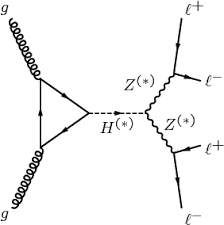
\includegraphics[width=0.48\textwidth,angle=0]{Figures/ggH_feynman.png}
      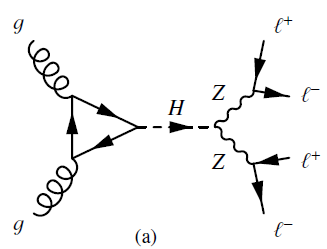
\includegraphics[width=0.45\textwidth,angle=0]{Figures/ggH_feynman2.png}
    \caption{$\ggH$ process feynman diagram.}
  \label{fig:ggZZ_box}
  \end{center}
\end{figure}
%%%%%%%%
 
%All SM production modes have been produced individually to approximate the dependence of measurements on underlying assumptions of Higgs production mechanism. 
%We have also simulated a wide range of samples that provide descriptions for exotic Higgs-like resonances productions and their decay to the four-lepton final state to estimate the dependence of the measurements on the Higgs boson properties. These include spin-zero, spin-one
%and spin-two resonances with anomalous interactions with a pair of neutral gauge bosons ($ZZ$, $Z\gamma^{*}$, $\gamma^{*}\gamma^{*}$) described by
%higher-order operators, as discussed in details in Ref.~\cite{Khachatryan:2014kca}. 
%Produced samples, for each production mode, are also used to asses model dependence of measured results as shown in the Table ~\ref{tab:Accept_Eff_fOut}.
%The details of the method used to asses the model dependence will be
%described in Section \ref{sec:Systematics}. 
All these MC samples are produced using {\sc powheg} 
for the representation of QCD effects at NLO in Higgs production, and by using {\sc JHUgen}~\cite{Gao:2010qx,Bolognesi:2012mm,Anderson:2013afp} to 
represent such exotic resonances decays to four-leptons containing all the spin correlations.
\par
%The list of Standard Model Higgs boson  samples at $\sqrt{s} = 8$~TeV with corresponding values of cross sections can be found in Table~\ref{tab:MCsamplesSig}, 
%while all the signal MC samples studied in the analysis are listed in the Table~\ref{tab:samplesSM}. 
%A subset of these samples are used to asses the model dependence of the measurement results are indicated in the Table \ref{tab:Accept_Eff_fOut}.
%In a similar way, the samples of the exotic spin-parity models and exotic production/decay modes are presented in Table~\ref{tab:samplesExo} in 
%Appendix~\ref{app:samples}.
%\begin{table}[!h!tb]
%\begin{center}
%\small
%\caption{
%Standard Model signal Model Carlo samples studies in the analysis.
%Samples used for the estimation of the model dependence of the measurement results are denoted in the column ``D.''.
%\label{tab:samplesSM}
%}
%\begin{tabular}{|l|c|c|} \hline
%Sample & Description & D. \\ \hline
%SMHiggsToZZTo4L\_M-125\_8TeV-powheg15-JHUgenV3-pythia6 & gg$\rightarrow$H ({\sc powheg+JHU}) & Y \\
% SMHiggsToZZTo4L\_M-126\_8TeV-powheg15-JHUgenV3-pythia6 & gg$\rightarrow$H ({\sc powheg+JHU}) & Y \\
% GluGluToHToZZTo4L\_M-125\_8TeV-powheg15-pythia6 & gg$\rightarrow$H ({\sc powheg})& No \\
% GluGluToHToZZTo4L\_M-126\_8TeV-powheg15-pythia6 & gg$\rightarrow$H ({\sc powheg}) & No \\
% GluGluToHToZZTo4L\_M-125\_8TeV-powheg-pythia6 & gg$\rightarrow$H ({\sc powheg1.0})  & No \\
% GluGluToHToZZTo4L\_M-126\_8TeV-powheg-pythia6 & gg$\rightarrow$H ({\sc powheg1.0})  & No \\
% GluGluToHToZZTo4L\_M-125\_8TeV-minloHJJ-pythia6-tauola & gg$\rightarrow$H ({\sc minloHJJ}) & Y\\
% GluGluToHToZZTo4L\_M-126\_8TeV-minloHJJ-pythia6-tauola & gg$\rightarrow$H ({\sc minloHJJ}) & Y\\
% VBF\_HToZZTo4L\_M-125\_8TeV-powheg-pythia6 & VBF ({\sc powheg})& Y \\
% VBF\_HToZZTo4L\_M-126\_8TeV-powheg-pythia6 & VBF ({\sc powheg})& Y \\
% WH\_HToZZTo4L\_M-125\_8TeV-pythia6 & WH ({\sc pythia}) & Y \\
% WH\_HToZZTo4L\_M-126\_8TeV-pythia6 & WH ({\sc pythia})  & Y \\
% ZH\_HToZZTo4L\_M-125\_8TeV-pythia6 & ZH ({\sc pythia}) & Y \\
% ZH\_HToZZTo4L\_M-126\_8TeV-pythia6 & ZH ({\sc pythia}) & Y \\
% TTbarH\_HToZZTo4L\_M-125\_8TeV-pythia6 & ttH ({\sc pythia})& Y \\
% TTbarH\_HToZZTo4L\_M-126\_8TeV-pythia6 & ttH ({\sc pythia}) & Y \\
%\hline
%\end{tabular}
%\normalsize
%\end{center}
%\end{table}
\subsubsection{Background Samples}
For the estimations of the backgrounds, {\sc powheg V2} interfaced with {\sc pythia8} was used to generate the dominant process $\Pq\Paq \to \Z \Z \to 4\ell$  at the NLO accuracy level containing
s-, t- and u-channel diagrams ~\cite{Nason:2013ydw}. Generators were used with same configurations as used for the Higgs signal. Feynman diagrams of the involved background processes are shown in the Figure \ref{fig:ZZ_feynman}.
%with the same configurations as for the Higgs signal. 
The dynamical renormalization and factorization scales have been chosed equal to $m_{\Z\Z}$ since the simulation covers a wide range of invariant masses of ZZ.
%As this simulation covers a large
%range of ZZ invariant masses, dynamical QCD factorization and renormalization
%scales have been chosen, equal to $m_{\Z\Z}$. 

The $\Pg\Pg \! \to \! ZZ$ process (having about 4\% contribution to overall background yield), as shown in the Figure \ref{fig:ggZZ_box:c} is simulated at leading order (LO) 
with MCFM~\cite{MCFM,Campbell:2013una}. 
In order to have matching in spectra of $\Pg\Pg \! \to \mathrm{H} \to \! ZZ$ as predicted at NLO by {\sc powheg}, the showering of these samples has been performed with some different {\sc pythia8} settings.
This only allows emissions only up to parton-level scale (``wimpy'' shower).

%Although not directly used to model data observations, additional 
%MC samples of W$\cPZ$, Drell-Yan+jets, \ttbar, and tribosons are
%generated using {\sc MadGraph5\_aMCatNLO}~\cite{Alwall:2014hca} either
%inclusively or merging several jet multiplicities, as detailed in the table.

%, while the background process $\Pg\Pg \rightarrow \Z\Z \to 4\ell$ (Figure~\ref{fig:ggZZ_box}) was 
%generated using {\sc MCFM 6.7}.

\begin{figure}[!htb]
  \begin{center}
    \subfigure[s-channel]{
      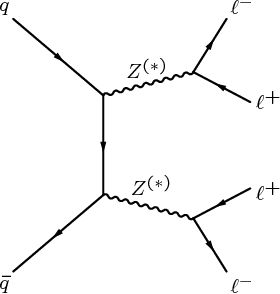
\includegraphics[width=0.3\textwidth,angle=0]{Figures/figures_feynman-qqZZ-t.png}
       \label{fig:qqZZ_feynman-t:a}
    }
    \subfigure[t-channel]{
      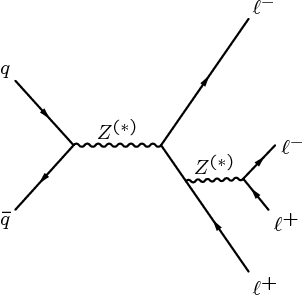
\includegraphics[width=0.3\textwidth,angle=0]{Figures/figures_feynman-qqZZ-s.png}
       \label{fig:qqZZ_feynman-t:b}
    } 
    \subfigure[ggZZ-box]{
      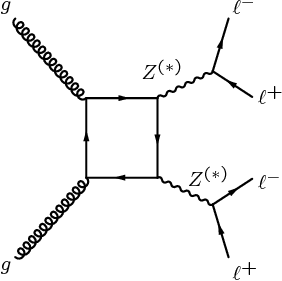
\includegraphics[width=0.3\textwidth,angle=0]{Figures/figures_feynman-ggbox.png}
       \label{fig:ggZZ_box:c}
    }   
	  \caption{$\Pq\Paq to \Z \Z \to 4\ell$  process s- and t- channel fynman diagrams (a) and (b). $\Pg\Pg \rightarrow \Z\Z \to 4\ell$  process fynman diagram (c).}
  \label{fig:ZZ_feynman}
  \end{center}
\end{figure}
%%%%%%%%
%\begin{figure}[!htb]
%  \begin{center}
%      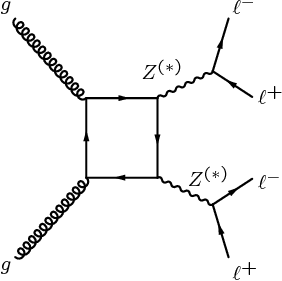
\includegraphics[width=0.28\textwidth,angle=0]{Figures/figures_feynman-ggbox.png}
%    \caption{$\Pg\Pg \rightarrow \Z\Z \to 4\ell$  process fynman diagram.}
%  \label{fig:ggZZ_box}
%  \end{center}
%\end{figure}
%%%%%%%%

\par 
The initial-state and final-state radiations are included for all events generators, which provides hints for the existence of extra (hard) photons in the event. 
Interference between all amplitudes of process $H \rightarrow 4\ell$ are properly taken into consideration both in {\sc powheg} and the {\sc JHUgen}.
%The {\sc powheg} and {\sc JHUgen} event generators also properly take into account interference between 
%all contributing amplitudes of the $H \rightarrow 4\ell$ process, containing those affiliated to the reordering of identical leptons
%in the $4\mu$ and $4e$ final states.
%For the generators, the used default parton distribution functions (PDFs) are NNPDF31_nlo_hessian_pdfas and NNPDF31_lo_as_0130  (at NLO and LO) are used.
For the generators, the used default parton distribution functions (PDFs) are NNPDF3.1 NLO (at NLO and LO) are used.
%The set of parton distribution functions (PDF) \textsc{cteq6l}~\cite{cteq66}, \textsc{CT10}~\cite{CT10}
%and \textsc{MSTW2008}~\cite{MSTW08} are used for LO, NLO, and NNLO generators.
\par
%The generated events were interfaced to {\sc pythia 8.209} Tune $Z2^{*}$~\cite{Chatrchyan:2011id} which follows CTEQ6L, to include the fact of the parton shower, underlying events and hadronization.
The generated events were interfaced to {\sc pythia 8.209} Tune tune CUETP8M1 to include the fact of the parton shower, underlying events and hadronization.
%, all generated events  were interfaced
% to {\sc pythia 6.4} Tune $Z2^{*}$~\cite{Chatrchyan:2011id}. 
%The {\sc pythia 6.4} $Z2^*$ tune is obtained from the Z1 tune~\cite{Field:2010bc}, that takes  the CTEQ5L parton distribution set, whereas $Z2^*$ follows CTEQ6L~\cite{Pumplin:2002vw}. {\sc HRes} does not supply  an interface with the programs
% that can include the effects of hadronization and multi-parton interaction. To correct {\sc HRes} predictions for these effects, the {\sc powheg+JHUgen}
% events without hadronization and  multi-parton interactions were reweighted to match closely the {\sc HRes} events in a  phase space minimally 
% greater than fiducial phase space. 
% After that, the hadronization and multi-parton interaction effects are included in reweighted
% {\sc powheg+JHUgen} events by an interface with {\sc pythia}. The procedure of reweighting events to match {\sc HRes} to add non-perturbative effects 
% to {\sc HRes} partonic level predictions was
%  repeated for all studied observables for integrated and differential cross section measurements. 
 \par
Processing of all generated events was made via a  full simulation for CMS detector using \textsc{GEANT4} ~\cite{GEANT} and their reconstruction was done by exploiting same algorithms used for the data analysis.
%were reconstructed with the same algorithms that are used for data analysis. 
Multiple proton-proton interactions are incorporated in the simulations by reweighting the pileup distribution to match the  distribution of the observed data. 
%While measuring the energy of jets and isolation of objects (using \textsc{FastJet} technique) ~\cite{Cacciari:2007fd,Cacciari:2008gn,Cacciari:2011ma}, the energy deposits from pileup interactions and  underlying events are subtracted.
%when computing the energy of jets and isolation of reconstructed objects using the \textsc{FastJet} technique~\cite{Cacciari:2007fd,Cacciari:2008gn,Cacciari:2011ma}.
%This technique is based on the calculation of the $\eta$-dependent average energy density %($\rho$), evaluated individually for each event.
%\par
%All the data-to-MC scale factors are  computed by using a ``T\&P'' technique \cite{CMS:2011lsa}, as described in Sections \ref{sec:eleEffMeas} and \ref{sec:muonEffMeas}, and  are used to correct simulated samples to compensate the differences
%of leptons' selection efficiencies in the data and MC simulation. There is negligibe dependence of the selection efficiencies used in the analysis over the primary vertices.
%%The dependency of the selection efficiency on the
%%number of reconstructed primary vertices in the event is found to be negligible for data samples.
%More details are presented and discussed in Ref.~\cite{Chatrchyan:2013mxa}.

\subsubsection{Pileup Reweighting}

For each year, corresponding simulation samples are reweighted to meet pileup distribution in the data. An example of the reweighting procedure for 2018 data is
shown in Figure \ref{fig:puWeight2018}.
%=======
\begin{figure}[!htb]
       \vspace*{0.3cm}
       \begin{center}
               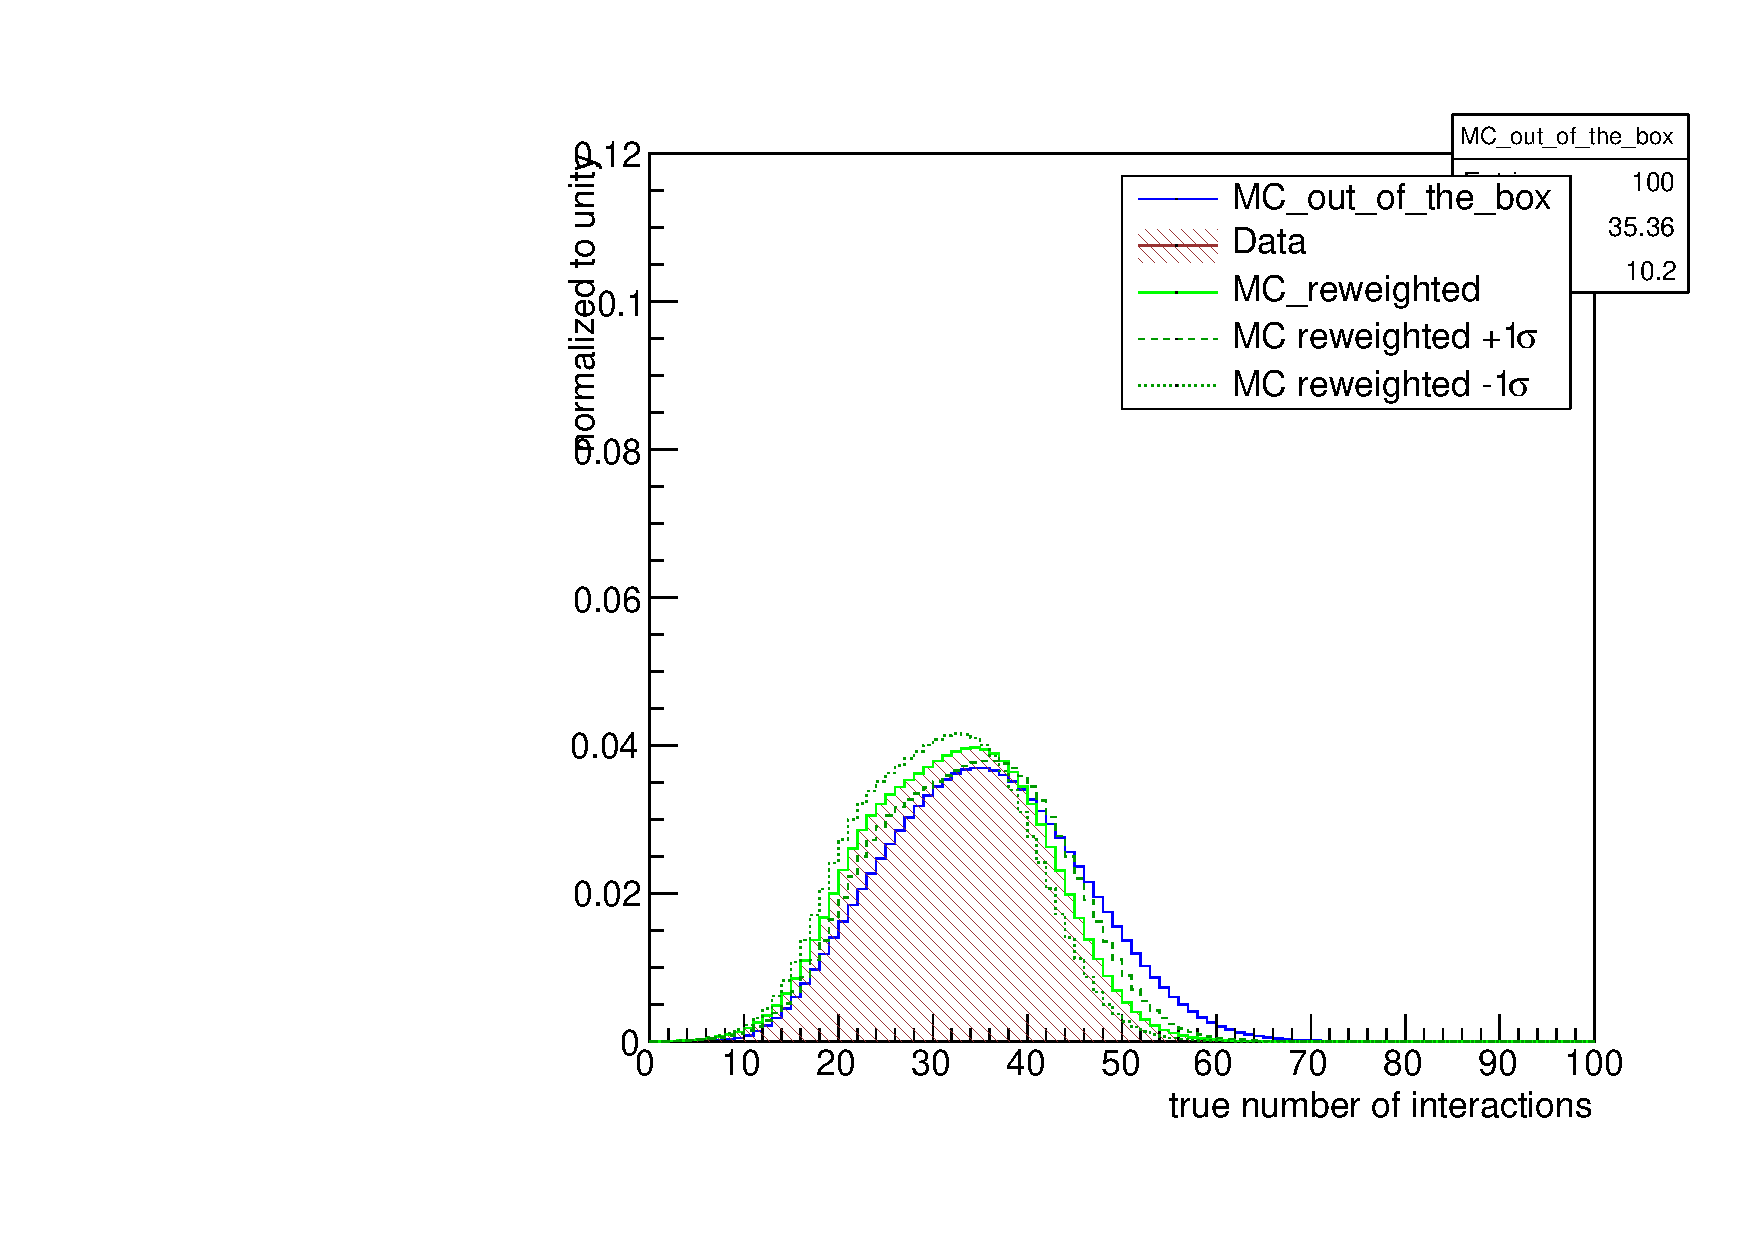
\includegraphics[width=0.45\textwidth]{Figures/PileUp/PileUp_2018.pdf} 
               \caption{Pileup distribution in 2018 MC and Data shown before and after the application of PU weights. Up and down variations of 5\% in the minimum bias
                       cross section when calculating the weighs are also shown.
                       \label{fig:puWeight2018}}
       \end{center}
\end{figure}
%%=======




%%%%%%%%%%
%%
%\begin{table}[htb]
%%
%  \begin{center}
%  \vspace*{0.3cm}
%
%    \begin{tabular}{llll}
%\hline %---------------------------------------------------------------------------------------------------------------------------------------------------------------------------- 
%\small      \bf{Process}                & \small \bf{MC}                        & \small\boldmath{$\sigma_{(N)NLO} $} &  Comment \\
%\hline \hline%==============================================================================================
%\small          gg$\rightarrow {\rm H}(\rightarrow {\rm Z}{\rm Z}) \rightarrow 4\ell$                   & \small{\sc powheg+JHUgen}     & \small 19.27  pb      & gg$\rightarrow$H production\\
%\small          ${qq} \rightarrow {\rm H}(\rightarrow {\rm Z}{\rm Z})+qq \rightarrow 4\ell+$X   & \small{\sc powheg}    & \small 1.578 pb       & VBF production\\
%\small          ${qq} \rightarrow {\rm H}(\rightarrow {\rm Z}{\rm Z})+W \rightarrow 4\ell+$X    & \small{\sc pythia}    & \small  0.7046 pb     & WH production\\
%\small          ${qq} \rightarrow {\rm H}(\rightarrow {\rm Z}{\rm Z})+Z \rightarrow 4\ell+$X            & \small{\sc pythia}    & \small 0.4153 pb      & ZH production\\
%\small          ${qq} \rightarrow {\rm H}(\rightarrow {\rm Z}{\rm Z})+t\bar{t} \rightarrow 4\ell+$X     & \small{\sc pythia}    & \small 0.1293 pb      & ttH production\\
%%\hline %---------------------------------------------------------------------------------------------------------------------------------------------------------------------------- 
%%\small         ${gg} \rightarrow {\rm H} \rightarrow {\rm Z}{\rm \gamma*} \rightarrow 4\ell $          & \small{\tt powheg + JHUGen}   & \small ?  fb  & Z$\gamma*$ decay\\
%%\small         ${gg} \rightarrow {\rm H} \rightarrow {\rm \gamma*}{\rm \gamma*} \rightarrow 4\ell $    & \small{\tt powheg + JHUGen}   & \small ?  fb  & $\gamma*\gamma*$ decay\\
%\hline %---------------------------------------------------------------------------------------------------------------------------------------------------------------------------- 
%   \end{tabular}
%
%  \end{center}
%%
%  \small
%  \caption{  MC simulation samples used for the signal processes predicted by the SM for 
%  m(H)=125.0$\GeV$ (${\rm Z}$ stands for ${\rm Z}$, ${\rm Z}^*$, $\gamma^*$). The cross sections
%  do not include the ZZ and $4\ell$ branching ratios. In the SM, the branching ratio
%  ${\rm H} \rightarrow {\rm Z}{\rm Z}\rightarrow 4\ell$ is 1.247$\times 10^{-4}$ for m(H)=125.0 $\GeV$.}
%  \label{tab:MCsamplesSig}
%%
%\end{table}
%%%%%%%
%\begin{table}[htb]
%%
%  \begin{center}
%  \vspace*{0.3cm}
%
%    \begin{tabular}{llll}
%\hline %---------------------------------------------------------------------------------------------------------------------------------------------------------------------------- 
%\small      \bf{Process}                & \small \bf{MC}                        & \small\boldmath{$\sigma_{(N)NLO} $} &  Comment \\
%\hline \hline%==============================================================================================
%\small          $ q\bar{q} \rightarrow {\rm Z}{\rm Z} \rightarrow 4e(4\mu,4\tau) $        & \small{\sc powheg}  & \small 76.91 fb       & s+t/u channels\\
%\small  $ q\bar{q} \rightarrow {\rm Z}{\rm Z} \rightarrow 2e2\mu  $             & \small{\sc powheg}            & \small 176.7 fb       & s+t/u channels\\
%\small  $ q\bar{q} \rightarrow {\rm Z}{\rm Z} \rightarrow 2e(2\mu)2\tau  $       & \small{\sc powheg}           & \small 176.7 fb       & s+t/u channels\\
%\small          $ q\bar{q} \rightarrow {\rm Z}{\rm Z} \rightarrow 4e $                           & \small{\sc powheg}   & \small 494.8 fb       & t/u channels only, $m_{ll}>1GeV$\\
%\small  $ q\bar{q} \rightarrow {\rm Z}{\rm Z} \rightarrow 2e2\mu  $             & \small{\sc powheg}            & \small 1527 fb        & t/u channels only, $m_{ll}>1GeV$\\
%\small  $ q\bar{q} \rightarrow {\rm Z}{\rm Z} \rightarrow 4\mu  $                & \small{\sc powheg}   & \small 488.4 fb       & t/u channels only, $m_{ll}>1GeV$\\
%\small          ${gg} \rightarrow {\rm Z}{\rm Z} \rightarrow 2e2\mu $                           & \small{\sc MCFM 6.7}          & \small 2.444  fb      & K-factor of 2.66 included\\
%\small          ${gg} \rightarrow {\rm Z}{\rm Z} \rightarrow 4\mu$                              & \small{\sc MCFM 6.7}          & \small 1.222 fb       & K-factor of 2.66 included\\
%\small          ${gg} \rightarrow {\rm Z}{\rm Z} \rightarrow 4e$                                        & \small{\sc MCFM 6.7}          & \small 1.222 fb       & K-factor of 2.66 included\\
%\hline %---------------------------------------------------------------------------------------------------------------------------------------------------------------------------- 
%   \end{tabular}
%  \end{center}
%%
%  \small
%  \caption{  MC simulation samples used for the background processes (${\rm Z}$ stands for ${\rm Z}$, ${\rm Z}^*$, $\gamma^*$);
%  In MC samples with label ``t/u channels only'' only the t/u channels are simulated in the $qq \to 4\ell$ process and these samples are used for the $Z \to 4\ell$ analysis.
%  The ``t/u channels only'' samples have lower cut in $m_{ll}$ of 1 GeV, while all other $qq \to ZZ$ and $gg \to ZZ$ samples have lower cut in $m_{ll}$ of 4 GeV. In case of 
%  the $gg \to ZZ$ background, the overall NLO k-factor of 2.66 is included, as discussed in Section~\ref{sec:EventsBackgrounds}.}
%  \label{tab:MCsamplesBkg}
%%
%\end{table}
